\documentclass{standalone}
\usepackage{tikz}
\usetikzlibrary{patterns, positioning}


\begin{document}
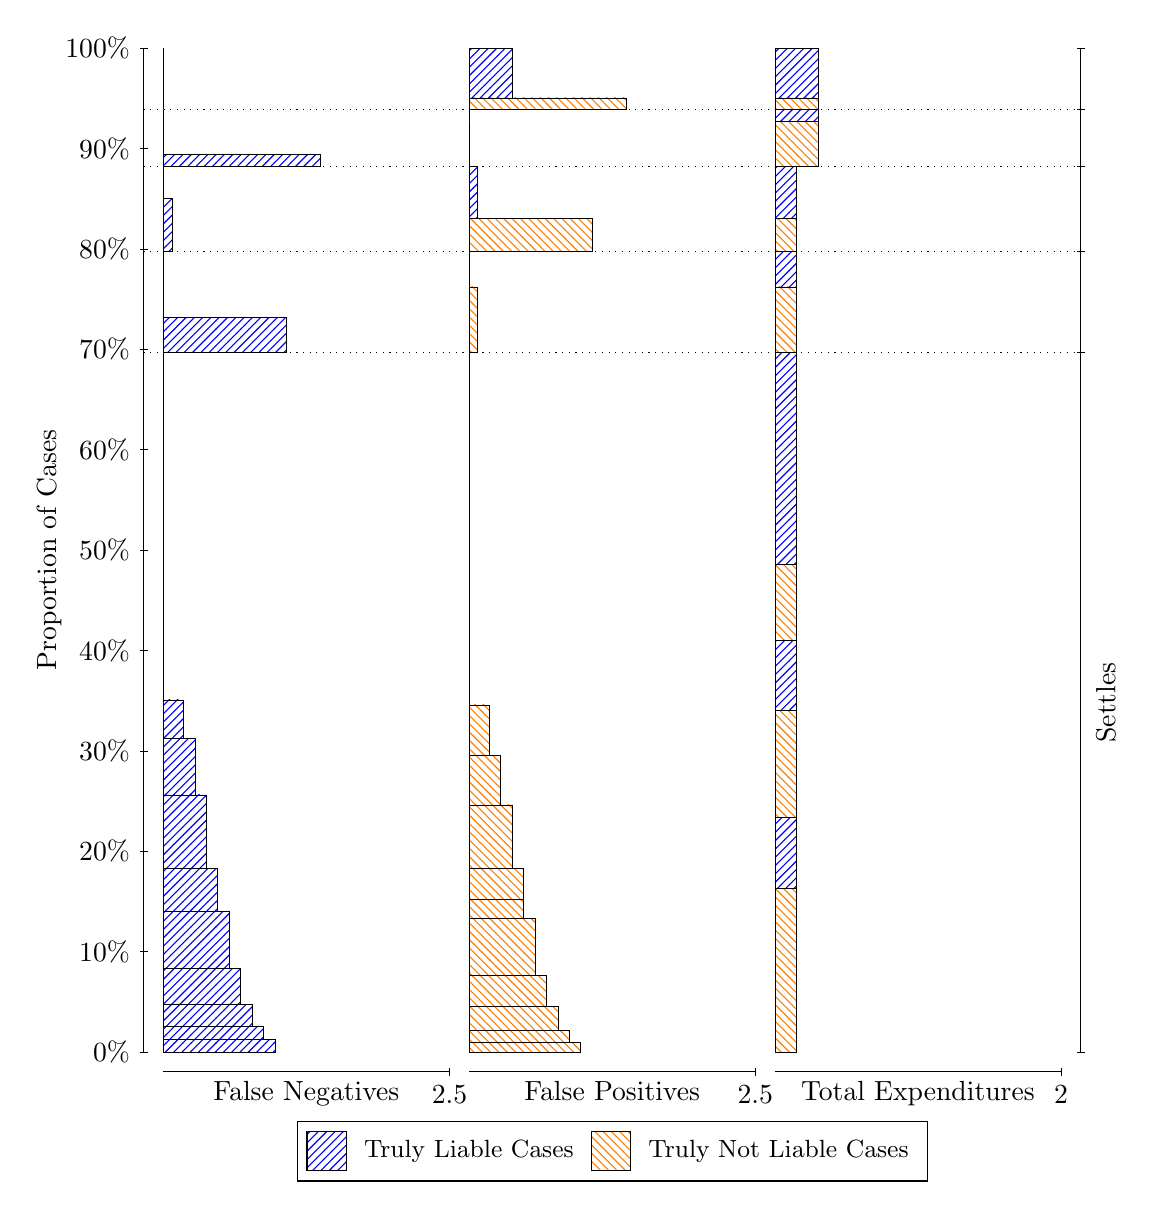
\begin{tikzpicture}
\draw[black, very thin] (1.5,1.75) -- (1.5,14.5);
\node[rotate=90, text=black, anchor=center] at (0.3, 8.125) {Proportion of Cases};
\draw[black, very thin] (1.45,1.75) -- (1.55,1.75);
\node[text=black, anchor=east] at (1.45, 1.75) {0\%};
\draw[black, very thin] (1.45,3.025) -- (1.55,3.025);
\node[text=black, anchor=east] at (1.45, 3.025) {10\%};
\draw[black, very thin] (1.45,4.3) -- (1.55,4.3);
\node[text=black, anchor=east] at (1.45, 4.3) {20\%};
\draw[black, very thin] (1.45,5.575) -- (1.55,5.575);
\node[text=black, anchor=east] at (1.45, 5.575) {30\%};
\draw[black, very thin] (1.45,6.85) -- (1.55,6.85);
\node[text=black, anchor=east] at (1.45, 6.85) {40\%};
\draw[black, very thin] (1.45,8.125) -- (1.55,8.125);
\node[text=black, anchor=east] at (1.45, 8.125) {50\%};
\draw[black, very thin] (1.45,9.4) -- (1.55,9.4);
\node[text=black, anchor=east] at (1.45, 9.4) {60\%};
\draw[black, very thin] (1.45,10.675) -- (1.55,10.675);
\node[text=black, anchor=east] at (1.45, 10.675) {70\%};
\draw[black, very thin] (1.45,11.95) -- (1.55,11.95);
\node[text=black, anchor=east] at (1.45, 11.95) {80\%};
\draw[black, very thin] (1.45,13.225) -- (1.55,13.225);
\node[text=black, anchor=east] at (1.45, 13.225) {90\%};
\draw[black, very thin] (1.45,14.5) -- (1.55,14.5);
\node[text=black, anchor=east] at (1.45, 14.5) {100\%};

\draw[black, very thin] (13.4,1.75) -- (13.4,14.5);
\draw[black, very thin] (13.35,1.75) -- (13.45,1.75);
\node[anchor=west] at (13.35, 1.75) {};
\draw[black, very thin] (13.35,10.63) -- (13.45,10.63);
\node[anchor=west] at (13.35, 10.63) {};
\draw[black, very thin] (13.35,11.919) -- (13.45,11.919);
\node[anchor=west] at (13.35, 11.919) {};
\draw[black, very thin] (13.35,13.001) -- (13.45,13.001);
\node[anchor=west] at (13.35, 13.001) {};
\draw[black, very thin] (13.35,13.717) -- (13.45,13.717);
\node[anchor=west] at (13.35, 13.717) {};
\draw[black, very thin] (13.35,14.5) -- (13.45,14.5);
\node[anchor=west] at (13.35, 14.5) {};

\draw[black, very thin, pattern color=blue, pattern=north east lines] (1.75,1.75) rectangle (3.167,1.9123);
\draw[black, very thin, pattern color=blue, pattern=north east lines] (1.75,1.9123) rectangle (3.0217,2.0737);
\draw[black, very thin, pattern color=blue, pattern=north east lines] (1.75,2.0737) rectangle (2.8763,2.3583);
\draw[black, very thin, pattern color=blue, pattern=north east lines] (1.75,2.3583) rectangle (2.731,2.8153);
\draw[black, very thin, pattern color=blue, pattern=north east lines] (1.75,2.8153) rectangle (2.5857,3.5347);
\draw[black, very thin, pattern color=blue, pattern=north east lines] (1.75,3.5347) rectangle (2.4403,4.0864);
\draw[black, very thin, pattern color=blue, pattern=north east lines] (1.75,4.0864) rectangle (2.295,5.0161);
\draw[black, very thin, pattern color=blue, pattern=north east lines] (1.75,5.0161) rectangle (2.1497,5.7306);
\draw[black, very thin, pattern color=blue, pattern=north east lines] (1.75,5.7306) rectangle (2.0043,6.2212);
\draw[black, very thin, pattern color=orange, pattern=north west lines] (1.75,6.2212) rectangle (1.75,10.63);
\draw[black, very thin, pattern color=blue, pattern=north east lines] (1.75,10.63) rectangle (3.3123,11.082);
\draw[black, very thin, pattern color=orange, pattern=north west lines] (1.75,11.082) rectangle (1.75,11.919);
\draw[black, very thin, pattern color=blue, pattern=north east lines] (1.75,11.919) rectangle (1.859,12.588);
\draw[black, very thin, pattern color=orange, pattern=north west lines] (1.75,12.588) rectangle (1.75,13.001);
\draw[black, very thin, pattern color=blue, pattern=north east lines] (1.75,13.001) rectangle (3.7483,13.152);
\draw[black, very thin, pattern color=orange, pattern=north west lines] (1.75,13.152) rectangle (1.75,13.717);
\draw[black, very thin, pattern color=orange, pattern=north west lines] (1.75,13.717) rectangle (1.75,13.868);
\draw[black, very thin, pattern color=blue, pattern=north east lines] (1.75,13.868) rectangle (1.75,14.5);
\draw[black, very thin, pattern color=orange, pattern=north west lines] (5.6333,1.75) rectangle (7.0503,1.8682);
\draw[black, very thin, pattern color=orange, pattern=north west lines] (5.6333,1.8682) rectangle (6.905,2.0266);
\draw[black, very thin, pattern color=orange, pattern=north west lines] (5.6333,2.0266) rectangle (6.7597,2.3276);
\draw[black, very thin, pattern color=orange, pattern=north west lines] (5.6333,2.3276) rectangle (6.6143,2.7195);
\draw[black, very thin, pattern color=orange, pattern=north west lines] (5.6333,2.7195) rectangle (6.469,3.4443);
\draw[black, very thin, pattern color=orange, pattern=north west lines] (5.6333,3.4443) rectangle (6.3237,3.6833);
\draw[black, very thin, pattern color=orange, pattern=north west lines] (5.6333,3.6833) rectangle (6.3237,4.0832);
\draw[black, very thin, pattern color=orange, pattern=north west lines] (5.6333,4.0832) rectangle (6.1783,4.887);
\draw[black, very thin, pattern color=orange, pattern=north west lines] (5.6333,4.887) rectangle (6.033,5.5209);
\draw[black, very thin, pattern color=orange, pattern=north west lines] (5.6333,5.5209) rectangle (5.8877,6.1584);
\draw[black, very thin, pattern color=blue, pattern=north east lines] (5.6333,6.1584) rectangle (5.6333,10.63);
\draw[black, very thin, pattern color=orange, pattern=north west lines] (5.6333,10.63) rectangle (5.7423,11.467);
\draw[black, very thin, pattern color=blue, pattern=north east lines] (5.6333,11.467) rectangle (5.6333,11.919);
\draw[black, very thin, pattern color=orange, pattern=north west lines] (5.6333,11.919) rectangle (7.1957,12.332);
\draw[black, very thin, pattern color=blue, pattern=north east lines] (5.6333,12.332) rectangle (5.7423,13.001);
\draw[black, very thin, pattern color=orange, pattern=north west lines] (5.6333,13.001) rectangle (5.6333,13.566);
\draw[black, very thin, pattern color=blue, pattern=north east lines] (5.6333,13.566) rectangle (5.6333,13.717);
\draw[black, very thin, pattern color=orange, pattern=north west lines] (5.6333,13.717) rectangle (7.6317,13.868);
\draw[black, very thin, pattern color=blue, pattern=north east lines] (5.6333,13.868) rectangle (6.1783,14.5);
\draw[black, very thin, pattern color=orange, pattern=north west lines] (9.5167,1.75) rectangle (9.7892,3.8266);
\draw[black, very thin, pattern color=blue, pattern=north east lines] (9.5167,3.8266) rectangle (9.7892,4.7295);
\draw[black, very thin, pattern color=orange, pattern=north west lines] (9.5167,4.7295) rectangle (9.7892,6.0918);
\draw[black, very thin, pattern color=blue, pattern=north east lines] (9.5167,6.0918) rectangle (9.7892,6.9735);
\draw[black, very thin, pattern color=orange, pattern=north west lines] (9.5167,6.9735) rectangle (9.7892,7.943);
\draw[black, very thin, pattern color=blue, pattern=north east lines] (9.5167,7.943) rectangle (9.7892,10.63);
\draw[black, very thin, pattern color=orange, pattern=north west lines] (9.5167,10.63) rectangle (9.7892,11.467);
\draw[black, very thin, pattern color=blue, pattern=north east lines] (9.5167,11.467) rectangle (9.7892,11.919);
\draw[black, very thin, pattern color=orange, pattern=north west lines] (9.5167,11.919) rectangle (9.7892,12.332);
\draw[black, very thin, pattern color=blue, pattern=north east lines] (9.5167,12.332) rectangle (9.7892,13.001);
\draw[black, very thin, pattern color=orange, pattern=north west lines] (9.5167,13.001) rectangle (10.062,13.566);
\draw[black, very thin, pattern color=blue, pattern=north east lines] (9.5167,13.566) rectangle (10.062,13.717);
\draw[black, very thin, pattern color=orange, pattern=north west lines] (9.5167,13.717) rectangle (10.062,13.868);
\draw[black, very thin, pattern color=blue, pattern=north east lines] (9.5167,13.868) rectangle (10.062,14.5);
\draw[black, dotted] (1.5,10.63) -- (13.4,10.63);
\draw[black, dotted] (1.5,11.919) -- (13.4,11.919);
\draw[black, dotted] (1.5,13.001) -- (13.4,13.001);
\draw[black, dotted] (1.5,13.717) -- (13.4,13.717);
\draw[black, very thin] (1.75,1.5) -- (5.3833,1.5);
\node[text=black, anchor=north] at (3.5667, 1.5) {False Negatives};
\draw[black, very thin] (5.3833,1.45) -- (5.3833,1.55);
\node[text=black, anchor=north] at (5.3833, 1.45) {2.5};

\draw[black, very thin] (5.6333,1.5) -- (9.2667,1.5);
\node[text=black, anchor=north] at (7.45, 1.5) {False Positives};
\draw[black, very thin] (9.2667,1.45) -- (9.2667,1.55);
\node[text=black, anchor=north] at (9.2667, 1.45) {2.5};

\draw[black, very thin] (9.5167,1.5) -- (13.15,1.5);
\node[text=black, anchor=north] at (11.333, 1.5) {Total Expenditures};
\draw[black, very thin] (13.15,1.45) -- (13.15,1.55);
\node[text=black, anchor=north] at (13.15, 1.45) {2};

\node[text=black, centered, rotate=90] at (13.72, 6.1898) {Settles};





\draw (7.449999999999999,1.5) node[draw=none] (baseCoordinate) {};
\begin{scope}[align=center]
        \matrix[scale=0.5, draw=black, below=0.5cm of baseCoordinate, nodes={draw}, column sep=0.1cm]{
            \node[rectangle, draw, minimum width=0.5cm, minimum height=0.5cm, pattern color=blue, pattern=north east lines] {}; &
            \node[draw=none, font=\small, text=black] (B) {Truly Liable Cases}; &
            \node[rectangle, draw, minimum width=0.5cm, minimum height=0.5cm, pattern color=orange, pattern=north west lines] {}; &
            \node[draw=none, font=\small, text=black] (B) {Truly Not Liable Cases}; \\
            };
\end{scope}

\end{tikzpicture}
\end{document}